\subsection{Medición de la resistencia interna de un voltímetro}\label{sec:resistencia de volt}

\paragraph{}
En esta sección se midió la resistencia interna de un voltímetro. Para esto, se armó el circuito de la figura \ref{fig:esq_voltimetro}, utilizando una fuente constante, una resistencia variable y un voltímetro en paralelo.

\begin{figure}[H]
    \centering
    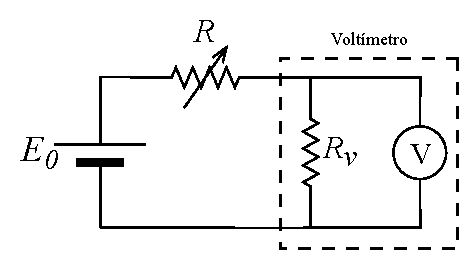
\includegraphics[width = 0.5\linewidth]{Esquemas/ResistenciaVoltimetro.pdf}
    \caption{Esquema que representa un circuito eléctrico formado por una fuente de voltaje constante $E_0$, una resistencia variable $R$ y un voltímetro conectados en serie. Este último está modelado como un voltímetro ideal conectado en paralelo con su resistencia interna $R_v$. $R$ es variable con el propósito de generar distintos voltajes para ser medidos. Esta configuración permite estudiar la relación entre voltaje y resistencia para finalmente determinar el valor de $R_v$.}
    \label{fig:esq_voltimetro}
\end{figure}
\paragraph{}
Se realizó un barrido de resistencias y se registró en cada caso la diferencia de potencial indicada por el voltímetro, manteniendo la escala de medición del mismo, dado que su resistencia interna puede variar con la escala. Además, se midió en cada caso y de manera independiente el valor de la resistencia.
\paragraph{}
Utilizando la ley de Ohm (Ec. \ref{eqn:ley de ohm}), se determinó que la caída de potencial $V_{R_v}$ a través de la resistencia del voltímetro ($R_v$) está dada por la ecuación  \ref{eqn:caida voltimetro}, donde $R$ es la resistencia variable y $E_0$ es la diferencia de potencial entregada por la fuente.

\begin{equation}\label{eqn:caida voltimetro}
    V_{R_v} = \frac{E_0 R_v}{R + R_v}
\end{equation}
\paragraph{}
Se realizó un ajuste mediante la ecuación \ref{eqn:caida voltimetro}, siendo $V_{R_v}$ la diferencia de potencial y $R$ la resistencia medida, y se obtuvo el gráfico de la figura \ref{fig:fig_voltimetro}.
\begin{figure}[H]
    \centering
    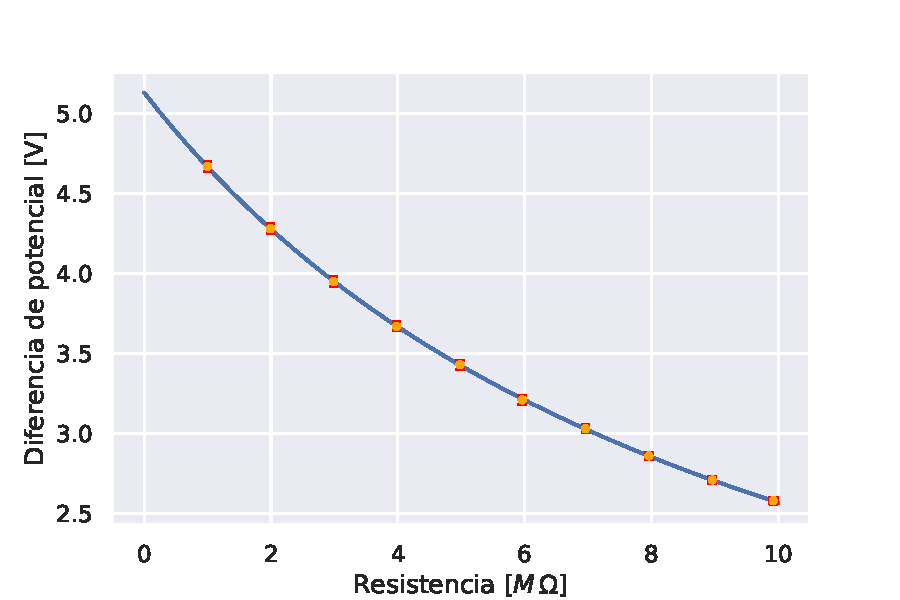
\includegraphics[width = 0.65\linewidth]{figuras/voltimetro.pdf}
    \caption{Ajuste por medio de la ecuación \ref{eqn:caida voltimetro} de las mediciones de voltaje en función del valor de la resistencia variable.}
    \label{fig:fig_voltimetro}
\end{figure}
\paragraph{}
 Se obtuvo un valor de $R_v=(10.01\pm0.02)$ M $\Omega$ para la resistencia interna del voltímetro. Este resultado coincide con el valor reportado por el fabricante. Además, se recuperó la diferencia de potencial aportada por la fuente cuando la resistencia es nula.
